% =====================================================================
%  MiniVPN -- Operating System Lab Project Report
%  Compile:  pdflatex report.tex   (run twice for contents/references)
%  Needs jiit-logo.png in the same folder.
% =====================================================================
\documentclass[12pt,a4paper]{report}

\usepackage[margin=1in]{geometry}
\usepackage{graphicx}
\usepackage{amsmath}
\usepackage{setspace}
\usepackage{enumitem}
\usepackage{booktabs}
\usepackage{tabularx}
\usepackage{longtable}
\usepackage{float}
\usepackage{xcolor}
\usepackage{listings}
\usepackage{tikz}
\usetikzlibrary{positioning,arrows.meta,shapes.geometric,fit,calc}
\usepackage[hidelinks]{hyperref}

\setstretch{1.3}
\setlist{itemsep=2pt,topsep=4pt}

% Running header and page number (no extra package needed).
% Chapter opening pages keep the plain style (page number only).
\makeatletter
\def\ps@project{%
  \def\@oddhead{\small MiniVPN -- OS Lab Project Report\hfill JIIT, Noida}%
  \let\@evenhead\@oddhead
  \def\@oddfoot{\hfil\thepage\hfil}%
  \let\@evenfoot\@oddfoot}
\makeatother
\pagestyle{project}

\definecolor{codebg}{RGB}{247,247,247}
\definecolor{codekw}{RGB}{0,0,160}
\definecolor{codecm}{RGB}{0,120,0}
\definecolor{codestr}{RGB}{160,30,30}
\lstset{
  language=C, basicstyle=\ttfamily\small, backgroundcolor=\color{codebg},
  keywordstyle=\color{codekw}\bfseries, commentstyle=\color{codecm}\itshape,
  stringstyle=\color{codestr}, frame=single, rulecolor=\color{black!25},
  breaklines=true, columns=fullflexible, numbers=left, numberstyle=\tiny\color{gray},
  xleftmargin=1.5em, framexleftmargin=1.5em, showstringspaces=false, tabsize=4,
  captionpos=b}

% ---------------------------------------------------------------------
%  Front-page details -- edit here
% ---------------------------------------------------------------------
\newcommand{\projecttitle}{MiniVPN: A Secure Self-Hosted Virtual Private Network Built on Linux Kernel Interfaces}
\newcommand{\doctype}{Operating System Lab Project Report}
\newcommand{\semester}{Semester 5}

\begin{document}

% =========================== FRONT PAGE ==============================
\begin{titlepage}
\centering
{\Large\bfseries BACHELOR OF TECHNOLOGY\par}
\vspace{1.2cm}

\includegraphics[width=4.2cm]{jiit-logo.png}\par
\vspace{0.6cm}
{\large Jaypee Institute of Information Technology, Noida\par}
\vspace{1.4cm}
{\LARGE\bfseries \projecttitle\par}
\vspace{1.2cm}
{\Large \semester\par}
\vspace{0.4cm}
{\Large\bfseries \doctype\par}
\vfill
\begin{minipage}[t]{0.52\textwidth}
\raggedright
{\large\bfseries Made By:}\\[6pt]
Sansriti Mishra \hfill 2401030293\\
Mokshi Mittal \hfill 2401030326\\
Sanvi Dhingra \hfill 2401030312
\end{minipage}%
\hfill
\begin{minipage}[t]{0.38\textwidth}
\raggedleft
{\large\bfseries Submitted To:}\\[6pt]
Dr. Sayani Ghoshal\\
Dr. Vikash\\
Dr. Tanvi Gautam
\end{minipage}
\vspace{1.5cm}

{\large Department of Computer Science \& Engineering and IT\par}
\end{titlepage}

% ======================== PRELIMINARY PAGES ==========================
\pagenumbering{roman}

\chapter*{Declaration}
\addcontentsline{toc}{chapter}{Declaration}
We hereby declare that the project titled \textbf{``\projecttitle''}, submitted as
part of the Operating System Lab in Semester 5 of the Bachelor of Technology programme
at Jaypee Institute of Information Technology, Noida, is our own work. It has not been
submitted elsewhere for any other degree or course. All sources used have been
acknowledged in the references.

\vspace{2cm}
\noindent
\begin{tabular}{@{}ll@{}}
Sansriti Mishra & 2401030293\\[4pt]
Mokshi Mittal & 2401030326\\[4pt]
Sanvi Dhingra & 2401030312
\end{tabular}

\vspace{1cm}
\noindent Date: \rule{4cm}{0.4pt}

\chapter*{Acknowledgement}
\addcontentsline{toc}{chapter}{Acknowledgement}
We thank our faculty, \textbf{Dr. Sayani Ghoshal}, \textbf{Dr. Vikash} and
\textbf{Dr. Tanvi Gautam}, for their guidance throughout the Operating System Lab.
Their lectures on processes, file systems, inter-process communication and
synchronisation gave us the foundation on which this project is built. We also thank
the Department of Computer Science \& Engineering and IT, JIIT Noida, for providing
the facilities and environment to carry out this work.

\chapter*{Abstract}
\addcontentsline{toc}{chapter}{Abstract}
This report presents \textbf{MiniVPN}, a virtual private network implemented from
scratch in C for Linux. MiniVPN connects devices such as laptops and servers into one
encrypted private network over the public Internet. Each device has its own key and a
fixed tunnel address, and an administrator can add, disable or revoke devices while
the server is running.

The project is designed around operating-system mechanisms. A TUN virtual network
device, created through \texttt{/dev/net/tun} and configured with \texttt{ioctl}, lets
a user-space process send and receive raw IP packets. A single-threaded event loop
built on \texttt{epoll} multiplexes the TUN device, a UDP socket, a Unix-domain
control socket, signals (through \texttt{signalfd}) and timers (through
\texttt{timerfd}). After setup the daemon drops root privileges. Administrative
tools communicate with it over a Unix-domain socket whose callers are authenticated
with \texttt{SO\_PEERCRED}, and shared files are updated atomically using
\texttt{flock}, \texttt{fsync} and \texttt{rename}.

Security is provided by an authenticated one-round-trip handshake using X25519 key
exchange and HKDF, a ChaCha20-Poly1305 data channel, a 1024-entry anti-replay window,
source-address anti-spoofing and periodic rekeying for forward secrecy. The system is
verified by 119 C unit checks (including published RFC test vectors), 13 Python tests
and 53 end-to-end checks that run across four Linux network namespaces. It reaches a
throughput of about 680 Mbit/s on a laptop.

\tableofcontents
\listoffigures
\listoftables

\clearpage
\pagenumbering{arabic}

% ============================ CHAPTERS ===============================

\chapter{Introduction}

\section{Background}
A \emph{Virtual Private Network} (VPN) creates a private network on top of a public
one. Packets that travel between members of the VPN are encapsulated inside other
packets, encrypted and authenticated. To applications, the remote machines appear to
be on the same local network.

VPNs are used by companies to connect remote employees to internal services, to link
office networks, and to protect traffic on untrusted Wi-Fi. Mature implementations
include IPsec, OpenVPN and WireGuard.

\section{Motivation}
A VPN is an ideal Operating System Lab project because it cannot be built without
working directly with the kernel. A VPN process must:
\begin{itemize}
  \item create a virtual network device and configure it (OS: device drivers, \texttt{ioctl});
  \item wait on several input sources at once without busy-waiting (OS: I/O multiplexing);
  \item react to signals and timers safely (OS: signals, timers, asynchronous events);
  \item run with the least privilege possible (OS: users, credentials, protection);
  \item communicate with management tools (OS: inter-process communication);
  \item share configuration files with other processes safely (OS: file locking, atomicity).
\end{itemize}
Writing every one of these pieces ourselves turns textbook concepts into working code
that can be tested and measured.

\section{Problem Statement}
Design and implement a secure, self-hosted VPN for Linux that connects multiple
devices to a central server. The VPN should let an administrator manage devices while
the server is running, and it should demonstrate core operating-system mechanisms in
its implementation.

\section{Objectives}
\begin{enumerate}
  \item Create and configure a TUN virtual interface from user space.
  \item Build an event-driven, single-threaded server and client using \texttt{epoll},
        \texttt{signalfd} and \texttt{timerfd}.
  \item Encapsulate IPv4 packets in UDP with authenticated encryption and forward secrecy.
  \item Run the daemon without root privileges after initialisation.
  \item Provide a local IPC control interface and an administration CLI and web dashboard.
  \item Validate the system with unit tests, end-to-end tests in network namespaces and
        memory-error sanitizers.
\end{enumerate}

\section{Organisation of the Report}
Chapter~\ref{ch:background} covers the background concepts. Chapter~\ref{ch:design}
describes the system architecture and protocol. Chapter~\ref{ch:impl} explains the
implementation, focusing on operating-system mechanisms. Chapter~\ref{ch:testing}
presents testing and results, and Chapter~\ref{ch:conclusion} concludes with
limitations and future work.

% ---------------------------------------------------------------------
\chapter{Background and Related Work}\label{ch:background}

\section{TUN/TAP Virtual Network Devices}
Linux provides the TUN/TAP driver, which creates network interfaces that are backed by
a user-space program instead of hardware. A \textbf{TUN} device works at layer 3 (IP
packets) and a \textbf{TAP} device works at layer 2 (Ethernet frames). A process opens
the character device \texttt{/dev/net/tun} and issues the \texttt{TUNSETIFF}
\texttt{ioctl}. From then on:
\begin{itemize}
  \item every packet the kernel routes to the interface can be read with \texttt{read()} on the file descriptor;
  \item every packet the process \texttt{write()}s is injected into the kernel network stack
        as if it had arrived on that interface.
\end{itemize}
The interface exists only while the file descriptor is open, so its lifetime is tied to
the process. MiniVPN uses TUN mode with \texttt{IFF\_NO\_PI} so that reads return bare
IPv4 packets.

\section{I/O Multiplexing}
A VPN must wait on several sources at once: the TUN device, the network socket, timers
and signals. Common designs are:
\begin{itemize}
  \item \textbf{one thread per source}, which needs locks around shared state;
  \item \textbf{\texttt{select}/\texttt{poll}}, which scan every descriptor on each call ($O(n)$);
  \item \textbf{\texttt{epoll}}, where the kernel keeps an interest list and returns only ready
        descriptors.
\end{itemize}
Linux also turns signals (\texttt{signalfd}) and timers (\texttt{timerfd}) into file
descriptors. A single \texttt{epoll\_wait} call can therefore handle every event in the
program, with no signal handlers running at unpredictable points and no threads to
synchronise.

\section{Cryptographic Building Blocks}
\begin{description}[style=nextline]
  \item[X25519 (RFC 7748)] Elliptic-curve Diffie--Hellman. Two parties exchange public
        keys and compute the same shared secret.
  \item[HKDF-SHA256 (RFC 5869)] Derives several independent keys from one shared secret.
  \item[HMAC-SHA256 (RFC 2104)] A keyed message authentication code, used to authenticate
        handshake messages.
  \item[ChaCha20-Poly1305 (RFC 8439)] Authenticated encryption with associated data (AEAD).
        It encrypts the payload and produces a 16-byte tag that detects any modification.
  \item[Ed25519 (RFC 8032)] A digital signature scheme, used to sign license files.
\end{description}

\section{Existing VPN Solutions}
\begin{table}[H]
\centering
\caption{Comparison with existing VPNs}
\begin{tabularx}{\textwidth}{@{}lXXX@{}}
\toprule
 & \textbf{OpenVPN} & \textbf{WireGuard} & \textbf{MiniVPN}\\
\midrule
Runs in & User space & Kernel module & User space\\
Transport & UDP or TCP & UDP & UDP\\
Crypto & TLS, configurable & Fixed modern suite & Fixed modern suite\\
Code size & $\sim$100k lines & $\sim$4k lines (kernel) & $\sim$3k lines C\\
Device management & Certificates (PKI) & Static public keys & Registry with live revoke\\
Built-in dashboard & No & No & Yes\\
\bottomrule
\end{tabularx}
\end{table}
MiniVPN follows WireGuard's philosophy of a small, fixed cryptographic design, but runs
in user space so that every OS mechanism is visible in the source code.

% ---------------------------------------------------------------------
\chapter{System Design}\label{ch:design}

\section{Architecture}

\begin{figure}[H]
\centering
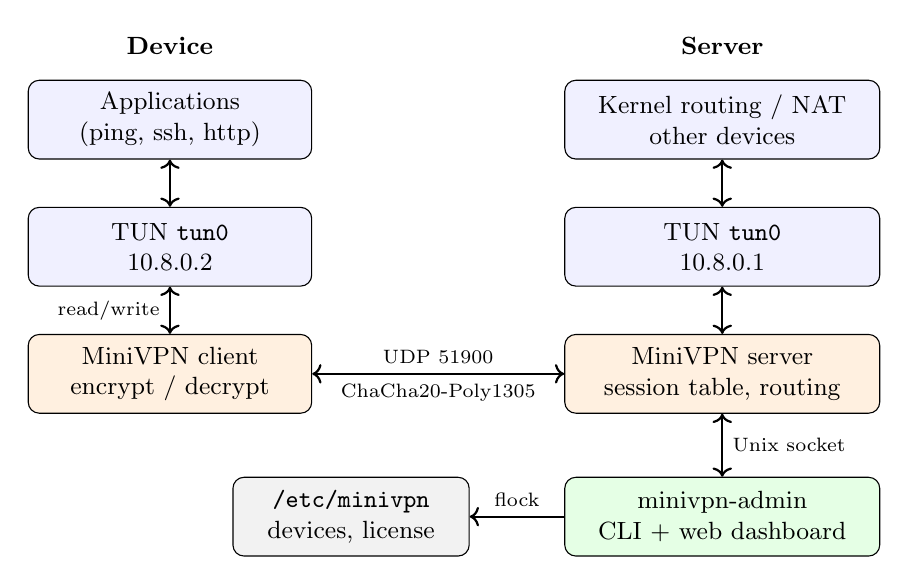
\begin{tikzpicture}[
  box/.style={draw,rounded corners,align=center,minimum height=1cm,font=\small,fill=blue!6},
  arr/.style={-{Stealth},thick}]
  \node[box,minimum width=3.6cm] (app) {Applications\\(ping, ssh, http)};
  \node[box,below=0.6cm of app,minimum width=3.6cm] (tun) {TUN \texttt{tun0}\\10.8.0.2};
  \node[box,below=0.6cm of tun,minimum width=3.6cm,fill=orange!12] (cli) {MiniVPN client\\encrypt / decrypt};
  \node[box,right=3.2cm of cli,minimum width=4cm,fill=orange!12] (srv) {MiniVPN server\\session table, routing};
  \node[box,above=0.6cm of srv,minimum width=4cm] (stun) {TUN \texttt{tun0}\\10.8.0.1};
  \node[box,above=0.6cm of stun,minimum width=4cm] (lan) {Kernel routing / NAT\\other devices};
  \node[box,below=0.8cm of srv,minimum width=4cm,fill=green!10] (adm) {minivpn-admin\\CLI + web dashboard};
  \node[box,left=1.2cm of adm,minimum width=3cm,fill=gray!10] (files) {\texttt{/etc/minivpn}\\devices, license};
  \draw[arr,<->] (app) -- (tun);
  \draw[arr,<->] (tun) -- node[left,font=\scriptsize]{read/write} (cli);
  \draw[arr,<->] (cli) -- node[above,font=\scriptsize]{UDP 51900}
                          node[below,font=\scriptsize]{ChaCha20-Poly1305} (srv);
  \draw[arr,<->] (srv) -- (stun);
  \draw[arr,<->] (stun) -- (lan);
  \draw[arr,<->] (adm) -- node[right,font=\scriptsize]{Unix socket} (srv);
  \draw[arr,->] (adm) -- node[above,font=\scriptsize]{flock} (files);
  \node[font=\small\bfseries,above=0.2cm of app] {Device};
  \node[font=\small\bfseries,above=0.2cm of lan] {Server};
\end{tikzpicture}
\caption{MiniVPN architecture}
\label{fig:arch}
\end{figure}

The system has three components (Table~\ref{tab:components}). The \emph{data plane} is
the C daemon, which runs in either server or client mode. The \emph{management plane} is
a Python tool with a command-line interface and a web dashboard. A separate vendor tool
signs license files and is never shipped.

\begin{table}[H]
\centering
\caption{Components}
\label{tab:components}
\begin{tabularx}{\textwidth}{@{}llX@{}}
\toprule
\textbf{Component} & \textbf{Language} & \textbf{Role}\\
\midrule
\texttt{minivpn} & C, OpenSSL & TUN device, encryption, sessions, routing, control socket\\
\texttt{minivpn-admin} & Python 3 (stdlib) & Device registry, configs, licenses, web dashboard\\
\texttt{license-tool} & C & Vendor-only license signing\\
\texttt{packaging/} & systemd, dpkg & Hardened services and \texttt{.deb} installer\\
\bottomrule
\end{tabularx}
\end{table}

\section{Packet Flow}
\begin{enumerate}
  \item An application on the device sends a packet to 10.8.0.1. The kernel's routing
        table sends it to \texttt{tun0}.
  \item The client's \texttt{epoll\_wait} reports the TUN descriptor as readable. The client
        reads the IPv4 packet.
  \item The client encrypts it with the client-to-server key, prepends a 16-byte header and
        sends it with \texttt{sendto()}.
  \item The server receives the datagram, finds the session by its id, checks the replay
        window and verifies the AEAD tag.
  \item The server checks that the inner IPv4 source address is the one assigned to that
        device (anti-spoofing) and writes the packet into its own \texttt{tun0}.
  \item The kernel delivers it locally, or forwards it to another device or to the Internet
        through NAT.
\end{enumerate}

\section{Source Code Organisation}
\begin{table}[H]
\centering
\caption{Source files}
\begin{tabularx}{\textwidth}{@{}lX@{}}
\toprule
\textbf{File} & \textbf{Responsibility}\\
\midrule
\texttt{server.c} & Session table, handshake, forwarding, reload and revocation, status JSON\\
\texttt{client.c} & Handshake state machine, reconnect, rekey, routes, full tunnel\\
\texttt{proto.c}, \texttt{channel.c}, \texttt{replay.c} & Wire format, key schedule, AEAD channel, anti-replay\\
\texttt{devices.c}, \texttt{license.c}, \texttt{config.c} & Device registry, signed licenses, config files\\
\texttt{tun.c} & TUN creation, address/MTU/route \texttt{ioctl}s\\
\texttt{sys.c} & \texttt{epoll}, \texttt{signalfd}, \texttt{timerfd}, privilege drop\\
\texttt{control.c} & Unix-domain control socket with peer-credential checks\\
\bottomrule
\end{tabularx}
\end{table}

\section{Protocol Design}

\subsection{Device identity and keys}
Each device has a public 16-byte \emph{device id} and a secret 32-byte \emph{device key},
both generated by \texttt{minivpn-admin add}. The keys are derived as:
\[
\begin{aligned}
\textit{auth\_key} &= \mathrm{HKDF}(\textit{device\_key},\ \text{``minivpn v2 handshake auth''})\\
k_{c2s} \,\|\, k_{s2c} &= \mathrm{HKDF}(\text{salt}=\textit{device\_key},\ \text{ikm}=\mathrm{X25519}(e_c, E_s),\ \text{info}=\ldots)
\end{aligned}
\]
An attacker needs both the device key and an ephemeral private key to read a session.
Ephemeral keys are wiped after the handshake, which gives \emph{forward secrecy}.

\subsection{Handshake}

\begin{figure}[H]
\centering
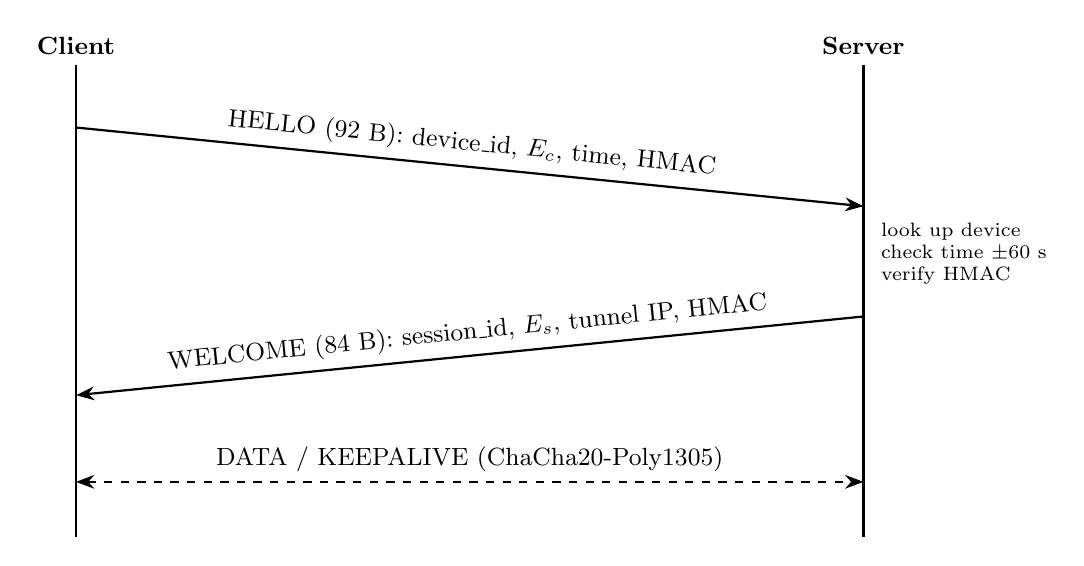
\begin{tikzpicture}[font=\small]
  \draw[thick] (0,0) node[above]{\textbf{Client}} -- (0,-6);
  \draw[thick] (10,0) node[above]{\textbf{Server}} -- (10,-6);
  \draw[-{Stealth},thick] (0,-0.8) -- node[above,sloped]{HELLO (92 B): device\_id, $E_c$, time, HMAC} (10,-1.8);
  \node[right,align=left,font=\scriptsize] at (10.1,-2.4) {look up device\\check time $\pm$60 s\\verify HMAC};
  \draw[-{Stealth},thick] (10,-3.2) -- node[above,sloped]{WELCOME (84 B): session\_id, $E_s$, tunnel IP, HMAC} (0,-4.2);
  \draw[{Stealth}-{Stealth},thick,dashed] (0,-5.3) -- node[above]{DATA / KEEPALIVE (ChaCha20-Poly1305)} (10,-5.3);
\end{tikzpicture}
\caption{One-round-trip handshake}
\label{fig:handshake}
\end{figure}

\begin{itemize}
  \item An unknown or disabled device, or a bad MAC, gets \textbf{no reply}, so scanners learn nothing.
  \item The timestamp must be within $\pm60$\,s, which limits replay of old HELLOs.
  \item The WELCOME MAC covers the HELLO's MAC, so a WELCOME is accepted only as the answer
        to the exact HELLO the client sent.
  \item A device holds one session. A new HELLO (rekey or reconnect) replaces the old one.
\end{itemize}

\subsection{Data packets}
\begin{table}[H]
\centering
\caption{Data packet format}
\begin{tabular}{@{}lll@{}}
\toprule
\textbf{Offset} & \textbf{Size} & \textbf{Field}\\
\midrule
0 & 1 & type: 3 DATA, 4 KEEPALIVE, 5 DISCONNECT\\
1 & 3 & reserved\\
4 & 4 & session id\\
8 & 8 & counter (also the nonce)\\
16 & $n$ & ChaCha20-Poly1305 ciphertext\\
$16+n$ & 16 & authentication tag\\
\bottomrule
\end{tabular}
\end{table}
The 16-byte header is authenticated as associated data but not encrypted. Each
direction uses its own key, so a nonce is never reused under the same key. The total
overhead is 32 bytes plus 28 bytes of UDP/IPv4 headers, so the default tunnel MTU of
1400 fits a 1500-byte path.

\subsection{Timers}
\begin{table}[H]
\centering
\caption{Protocol timers}
\begin{tabular}{@{}ll@{}}
\toprule
\textbf{Event} & \textbf{Value}\\
\midrule
Keepalive after idle & 10 s (both sides)\\
Client: server considered dead & 30 s without receiving\\
Server: session expires & 60 s without receiving\\
HELLO retransmission & 1, 2, 4, 8, 8, \ldots\ s (exponential backoff)\\
Rekey & every 300 s\\
\bottomrule
\end{tabular}
\end{table}

% ---------------------------------------------------------------------
\chapter{Implementation}\label{ch:impl}
This chapter describes how each operating-system concept is used in MiniVPN. Code
excerpts are taken directly from the source.

\section{Creating the TUN Device}
The daemon opens \texttt{/dev/net/tun} and asks the kernel to create an interface with
\texttt{TUNSETIFF}. The descriptor is opened non-blocking and close-on-exec.

\begin{lstlisting}[caption={Creating a TUN interface (\texttt{src/tun.c})}]
int tun_open(char name[IFNAMSIZ])
{
    int fd = open("/dev/net/tun", O_RDWR | O_NONBLOCK | O_CLOEXEC);
    if (fd < 0)
        return -1;

    struct ifreq ifr;
    memset(&ifr, 0, sizeof ifr);
    ifr.ifr_flags = IFF_TUN | IFF_NO_PI;
    snprintf(ifr.ifr_name, IFNAMSIZ, "%s", name);

    if (ioctl(fd, TUNSETIFF, &ifr) < 0) {
        close(fd);
        return -1;
    }
    snprintf(name, IFNAMSIZ, "%s", ifr.ifr_name);
    return fd;
}
\end{lstlisting}

The interface is then configured through \texttt{ioctl}s on an ordinary socket:
\texttt{SIOCSIFADDR} (address), \texttt{SIOCSIFNETMASK} (netmask), \texttt{SIOCSIFMTU}
(MTU) and \texttt{SIOCSIFFLAGS} (bring the link up). Routes are added with
\texttt{SIOCADDRT}. No external commands such as \texttt{ip} are run.

\paragraph{Full-tunnel routing.} To send all Internet traffic through the VPN without
deleting the existing default route, the client adds two routes, \texttt{0.0.0.0/1} and
\texttt{128.0.0.0/1}. By the longest-prefix-match rule they are more specific than the
default route \texttt{0.0.0.0/0}, so they win. A pinned host route to the server keeps
the encrypted UDP traffic itself on the real interface.

\section{Event Loop with \texttt{epoll}}
Both server and client run a single thread. All inputs are file descriptors registered
with one \texttt{epoll} instance:

\begin{table}[H]
\centering
\caption{Descriptors watched by the server's event loop}
\begin{tabular}{@{}ll@{}}
\toprule
\textbf{Descriptor} & \textbf{Event}\\
\midrule
UDP socket & encrypted packets from devices\\
TUN device & packets from the kernel to deliver to a device\\
\texttt{signalfd} & \texttt{SIGHUP} (reload), \texttt{SIGTERM}/\texttt{SIGINT} (exit), \texttt{SIGUSR1} (status)\\
\texttt{timerfd} & 1-second tick for keepalives and session expiry\\
control socket & commands from \texttt{minivpn-admin}\\
\bottomrule
\end{tabular}
\end{table}

\begin{lstlisting}[caption={Registering descriptors (\texttt{src/server.c})}]
if ((s.sigfd = make_signalfd()) < 0 || (s.timerfd = make_timerfd(1000)) < 0)
    goto out;
if ((s.ep = epoll_create1(EPOLL_CLOEXEC)) < 0)
    goto out;
if (epoll_watch(s.ep, s.udp) || epoll_watch(s.ep, s.tun) ||
    epoll_watch(s.ep, s.sigfd) || epoll_watch(s.ep, s.timerfd) ||
    (s.ctl >= 0 && epoll_watch(s.ep, s.ctl)))
    goto out;
\end{lstlisting}

Because there is only one thread, the session table needs no locks. To keep one busy
source from starving the others, each readiness event processes a bounded batch of
packets before returning to \texttt{epoll\_wait}.

\section{Signals as File Descriptors}
Traditional signal handlers run asynchronously and may only call async-signal-safe
functions. MiniVPN instead blocks the signals with \texttt{sigprocmask} and receives
them through \texttt{signalfd}, so they are handled synchronously in the main loop
like any other event.

\begin{lstlisting}[caption={Signal setup and handling (\texttt{src/sys.c}, \texttt{src/server.c})}]
sigset_t set;
sigemptyset(&set);
sigaddset(&set, SIGINT);  sigaddset(&set, SIGTERM);
sigaddset(&set, SIGHUP);  sigaddset(&set, SIGUSR1);
sigprocmask(SIG_BLOCK, &set, NULL);
int fd = signalfd(-1, &set, SFD_NONBLOCK | SFD_CLOEXEC);

/* in the event loop */
struct signalfd_siginfo si;
while (read(s->sigfd, &si, sizeof si) == (ssize_t)sizeof si) {
    switch (si.ssi_signo) {
    case SIGUSR1: print_status(s); break;
    case SIGHUP:  reload(s, NULL); break;
    default:      s->running = 0; break;
    }
}
\end{lstlisting}

\section{Timers}
A \texttt{timerfd} created on \texttt{CLOCK\_MONOTONIC} fires once a second. On each
tick the server expires idle sessions, and the client sends keepalives, retransmits
HELLOs with exponential backoff and starts a rekey every 300 seconds. A monotonic clock
is used so that changes to the wall-clock time cannot break the timers.

\section{Privilege Separation}
Creating a TUN device, setting addresses and binding the port need root
(\texttt{CAP\_NET\_ADMIN}). Processing untrusted network packets does not. Once setup is
complete, the server switches to an unprivileged user and checks that the change cannot
be undone:

\begin{lstlisting}[caption={Dropping privileges (\texttt{src/sys.c})}]
if (setgroups(0, NULL) < 0 || setgid(pw->pw_gid) < 0 ||
    setuid(pw->pw_uid) < 0)
    return -1;
if (pw->pw_uid != 0 && setuid(0) == 0) {
    log_error("privilege drop did not stick");
    return -1;
}
\end{lstlisting}
The order matters: supplementary groups and the group id must be dropped \emph{before}
the user id, because after \texttt{setuid} the process no longer has permission to
change them. Already-open descriptors (TUN, socket) remain usable after the drop, which
is the principle of least privilege in practice.

\section{Inter-Process Communication}
The administration tool controls the running server through a Unix-domain stream socket
(\texttt{/run/minivpn/control.sock}, mode 0600). The protocol is one text line in, one
JSON line out: \texttt{status}, \texttt{reload} or \texttt{kick <device-id>}.

The kernel reports the credentials of the connecting process through
\texttt{SO\_PEERCRED}. Only root or the daemon's own user is accepted:

\begin{lstlisting}[caption={Authenticating the caller (\texttt{src/control.c})}]
struct ucred cred;
socklen_t credlen = sizeof cred;
if (getsockopt(fd, SOL_SOCKET, SO_PEERCRED, &cred, &credlen) < 0 ||
    (cred.uid != 0 && cred.uid != geteuid())) {
    close(fd);
    return -1;
}
/* never let a stuck client block the data plane */
struct timeval tv = { .tv_sec = 0, .tv_usec = 500000 };
setsockopt(fd, SOL_SOCKET, SO_RCVTIMEO, &tv, sizeof tv);
\end{lstlisting}
Send and receive timeouts make sure a slow or malicious client cannot stall the
single-threaded event loop.

\section{File Locking and Atomic Updates}
The device registry \texttt{/etc/minivpn/devices} is written by the administration tool
(and possibly by several administrators at once) and read by the server on reload. To
keep it consistent:
\begin{enumerate}
  \item the writer takes an exclusive advisory lock with \texttt{flock};
  \item it writes the new content to a temporary file in the same directory;
  \item it calls \texttt{fsync} so the data reaches the disk;
  \item it calls \texttt{rename}, which atomically replaces the old file.
\end{enumerate}
A reader therefore always sees either the complete old file or the complete new file,
even if the system crashes in the middle of an update.

\section{Anti-Replay Window}
An attacker could record a valid encrypted packet and send it again. Each packet
carries a 64-bit counter, and the receiver keeps a 1024-bit sliding bitmap of counters
already seen. The window advances only \emph{after} the authentication tag has been
verified, so forged packets cannot move it.

\begin{lstlisting}[caption={Replay check (\texttt{src/replay.c})}]
int replay_check(const replay_window *w, uint64_t ctr)
{
    if (!w->seen_any || ctr > w->top)
        return 0;                      /* new, accept */
    if (w->top - ctr >= REPLAY_WINDOW)
        return -1;                     /* too old */
    return bit_get(w, ctr) ? -1 : 0;   /* duplicate? */
}
\end{lstlisting}

\section{Server Session Management}
The server keeps one session per device. A table indexed by tunnel IP gives
$O(1)$ lookup when routing packets from the TUN device to the correct device. When an
authenticated packet arrives from a new UDP address, the session's endpoint is updated,
which supports \emph{roaming} (for example, a laptop moving from Wi-Fi to a mobile
hotspot). On \texttt{reload}, the server re-reads the registry and the license and
immediately disconnects devices that were revoked or disabled.

\section{Management Plane}
\texttt{minivpn-admin} is written in Python using only the standard library. Its
commands are listed in Table~\ref{tab:admin}. The web dashboard (port 8090) shows
online devices, endpoints and live throughput, and protects administrative actions
with password hashing, session cookies, CSRF tokens, origin checks and login lockout.

\begin{table}[H]
\centering
\caption{Administration commands}
\label{tab:admin}
\begin{tabular}{@{}ll@{}}
\toprule
\textbf{Command} & \textbf{Action}\\
\midrule
\texttt{init} & create server config, device registry and dashboard password\\
\texttt{add <name>} & register a device and write its config file\\
\texttt{list}, \texttt{status} & show devices, online state and traffic\\
\texttt{disable}, \texttt{enable} & suspend or restore a device (keeps address and key)\\
\texttt{revoke} & delete a device permanently\\
\texttt{kick} & disconnect a device now\\
\texttt{license} & show or install a signed license\\
\texttt{audit} & show the administrator activity log\\
\texttt{web} & run the web dashboard\\
\bottomrule
\end{tabular}
\end{table}

\section{Deployment}
The project builds a Debian package with \texttt{make deb}. It installs systemd services
for the server, the dashboard and each client (\texttt{minivpn-client@<name>}). The
units use systemd sandboxing (restricted capabilities, read-only system directories,
private temporary directories) as an additional layer of OS-level protection.

% ---------------------------------------------------------------------
\chapter{Testing and Results}\label{ch:testing}

\section{Test Strategy}
\begin{table}[H]
\centering
\caption{Test suites}
\begin{tabularx}{\textwidth}{@{}lrX@{}}
\toprule
\textbf{Suite} & \textbf{Checks} & \textbf{Coverage}\\
\midrule
C unit tests (\texttt{make test}) & 119 & Crypto against RFC 4231, 5869, 7748 and 8032 test vectors; AEAD tampering; replay window; handshake binding; license verification; registry parsing\\
Python tests & 13 & Admin operations, device limits, password hashing, dashboard authentication, CSRF, origin checks, lockout\\
Integration (\texttt{make integration}) & 53 & End-to-end across 4 network namespaces (see below)\\
Sanitizers (\texttt{make sanitize}) & -- & All suites rebuilt with AddressSanitizer and UBSan\\
\bottomrule
\end{tabularx}
\end{table}

\section{Network Namespaces as a Test Bed}
A real VPN test needs several machines. Linux network namespaces give each process its
own interfaces, routing table and firewall, so one computer can simulate a server and
several devices. The integration script creates four namespaces connected by virtual
Ethernet (\texttt{veth}) pairs and runs a MiniVPN process in each.

\begin{figure}[H]
\centering
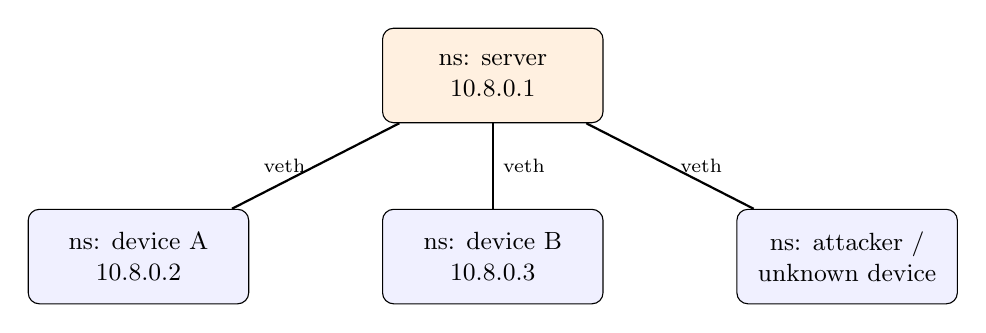
\begin{tikzpicture}[ns/.style={draw,rounded corners,minimum width=2.8cm,minimum height=1.2cm,align=center,font=\small,fill=blue!6}]
  \node[ns,fill=orange!12] (s) at (0,0) {ns: server\\10.8.0.1};
  \node[ns] (a) at (-4.5,-2.3) {ns: device A\\10.8.0.2};
  \node[ns] (b) at (0,-2.3) {ns: device B\\10.8.0.3};
  \node[ns] (c) at (4.5,-2.3) {ns: attacker /\\unknown device};
  \draw[thick] (s) -- node[left,font=\scriptsize]{veth} (a);
  \draw[thick] (s) -- node[right,font=\scriptsize]{veth} (b);
  \draw[thick] (s) -- node[right,font=\scriptsize]{veth} (c);
\end{tikzpicture}
\caption{Integration test topology}
\end{figure}

\section{Integration Test Scenarios}
\begin{longtable}{@{}p{5.5cm}p{9cm}@{}}
\caption{Selected end-to-end checks}\\
\toprule
\textbf{Scenario} & \textbf{Expected and observed result}\\
\midrule
\endfirsthead
\toprule
\textbf{Scenario} & \textbf{Expected and observed result}\\
\midrule
\endhead
Provisioning & Devices added with the admin tool connect and receive their fixed addresses\\
Wrong key / unknown device & Handshake gets no reply; no session is created\\
Encrypted wire & Packet capture on the underlay shows no plaintext payload\\
Bulk transfer & 8 MiB file transferred; SHA-256 matches on both sides\\
MTU & Maximum-size packets pass; oversize handling is correct\\
Kick, disable, enable, revoke & Each takes effect on the live server without restart\\
Rekey & New keys are installed and traffic counters are preserved\\
Device limit & Community limit (5 devices) enforced by both admin tool and server\\
Forged license & Rejected: signature verification fails\\
Business license & Applied with \texttt{reload}, no restart\\
Restart & Clients detect the dead server and reconnect automatically\\
Full tunnel & All traffic routed through the VPN via the \texttt{0/1} + \texttt{128/1} routes\\
\bottomrule
\end{longtable}

All 119 unit checks, 13 Python tests and 53 integration checks pass, and the sanitizer
builds report no memory errors or undefined behaviour.

\section{Performance}
Measured on a laptop, MiniVPN reaches approximately \textbf{680 Mbit/s} through the
encrypted tunnel. The per-packet overhead is 60 bytes (32 bytes MiniVPN header and
tag, 28 bytes UDP/IPv4). The main factors behind this throughput are the single-threaded
\texttt{epoll} design (no lock contention), non-blocking batched I/O, enlarged socket
buffers and the speed of ChaCha20-Poly1305 in software.

\section{Sample Output}
\begin{lstlisting}[language={},numbers=none,basicstyle=\ttfamily\scriptsize,caption={Administration CLI}]
$ sudo minivpn-admin add alice-laptop -o alice.conf
added alice-laptop (10.8.0.2); config written to alice.conf
server reloaded (3 device(s) active)

$ sudo minivpn-admin list
NAME           TUNNEL IP   STATUS  ONLINE  CONNECTED FROM       RECEIVED     SENT
alice-laptop   10.8.0.2    active  yes     49.36.112.7:55120      1.7 GB  394.9 MB
build-server   10.8.0.4    active  yes     34.93.10.4:51900      11.8 GB    8.5 GB
carol-phone    10.8.0.5    active  -       -                          -         -
\end{lstlisting}

% Add dashboard screenshots here, for example:
% \begin{figure}[H]
%   \centering
%   \includegraphics[width=\textwidth]{dashboard.png}
%   \caption{Web dashboard}
% \end{figure}

% ---------------------------------------------------------------------
\chapter{Conclusion and Future Work}\label{ch:conclusion}

\section{Conclusion}
MiniVPN is a complete, working VPN written from scratch in about 3{,}000 lines of C,
with a Python management plane. Building it required direct use of many
operating-system mechanisms: virtual devices and \texttt{ioctl}-based kernel
configuration, event-driven I/O with \texttt{epoll}, signals and timers as file
descriptors, privilege separation, Unix-domain IPC with credential checks, and atomic,
locked file updates. Together with authenticated encryption, replay protection and
forward secrecy, these produce a VPN that is secure, manageable while running, and
fast enough for real use. Extensive testing in network namespaces confirmed each
feature end to end.

\section{Limitations}
\begin{itemize}
  \item Clients run on Linux only.
  \item Only IPv4 is carried inside the tunnel.
  \item The dashboard has a single administrator account.
  \item The code has not been independently security-audited.
\end{itemize}

\section{Future Work}
\begin{itemize}
  \item Windows and macOS clients (Wintun driver, \texttt{utun} interface).
  \item IPv6 inside the tunnel.
  \item Multi-threaded data plane with \texttt{SO\_REUSEPORT} to use several CPU cores.
  \item Zero-copy I/O with \texttt{io\_uring} or batched \texttt{sendmmsg}/\texttt{recvmmsg}.
  \item Multiple administrator accounts with roles.
\end{itemize}

% ---------------------------------------------------------------------
\renewcommand{\bibname}{References}
\begin{thebibliography}{99}
\addcontentsline{toc}{chapter}{References}
\bibitem{tlpi} M. Kerrisk, \emph{The Linux Programming Interface}, No Starch Press, 2010.
\bibitem{osc} A. Silberschatz, P. B. Galvin, G. Gagne, \emph{Operating System Concepts}, 10th ed., Wiley, 2018.
\bibitem{tuntap} Linux kernel documentation, \emph{Universal TUN/TAP device driver}, \url{https://docs.kernel.org/networking/tuntap.html}.
\bibitem{epoll} Linux manual pages: \texttt{epoll(7)}, \texttt{signalfd(2)}, \texttt{timerfd\_create(2)}, \texttt{unix(7)}, \texttt{flock(2)}.
\bibitem{wg} J. A. Donenfeld, ``WireGuard: Next Generation Kernel Network Tunnel,'' in \emph{Proc. NDSS}, 2017.
\bibitem{rfc8439} Y. Nir, A. Langley, \emph{ChaCha20 and Poly1305 for IETF Protocols}, RFC 8439, 2018.
\bibitem{rfc7748} A. Langley, M. Hamburg, S. Turner, \emph{Elliptic Curves for Security}, RFC 7748, 2016.
\bibitem{rfc5869} H. Krawczyk, P. Eronen, \emph{HMAC-based Extract-and-Expand Key Derivation Function (HKDF)}, RFC 5869, 2010.
\bibitem{rfc8032} S. Josefsson, I. Liusvaara, \emph{Edwards-Curve Digital Signature Algorithm (EdDSA)}, RFC 8032, 2017.
\bibitem{rfc4303} S. Kent, \emph{IP Encapsulating Security Payload (ESP)}, RFC 4303, 2005 (anti-replay window).
\end{thebibliography}

% ---------------------------------------------------------------------
\appendix
\chapter{Build and Run Instructions}
\begin{lstlisting}[language=bash,numbers=none,caption={Quick demo on Linux or WSL2}]
sudo apt install build-essential libssl-dev python3
make
sudo ./scripts/demo.sh        # dashboard at http://localhost:8090
make test                     # unit tests
sudo make integration         # end-to-end tests
\end{lstlisting}

\begin{lstlisting}[language=bash,numbers=none,caption={Installing as a service}]
make deb
sudo apt install ./build/minivpn_2.0.0_amd64.deb
sudo minivpn-admin init --endpoint vpn.example.com
sudo minivpn-admin add laptop -o laptop.conf
sudo systemctl enable --now minivpn-server minivpn-admin
\end{lstlisting}

\end{document}
